\documentclass[a4]{scrartcl}

\usepackage[ngerman]{babel}
\usepackage[utf8]{inputenc}
\usepackage{mathtools}
\usepackage{amsmath}
\usepackage{amssymb}
\usepackage{geometry}
\usepackage{scrpage2}
\pagestyle{scrheadings}
\clearscrheadfoot


\geometry{
  paper=a4paper, % Change to letterpaper for US letter
  top=2cm, % Top margin
  bottom=1.5cm, % Bottom margin
  left=2cm, % Left margin
  right=3cm, % Right margin
  %showframe, % Uncomment to show how the type block is set on the page
}

\begin{document}

\subsection*{Vorlesung 4}

\textbf{Potenziale von IT - Traditionelle Perspektive}

\begin{itemize}
\item unstrukturierte Abläufe in routinemäßige Arbeit überführen
\item Beschleunigung
\item Ersatz und Reduktion menschlicher Arbeit
\item Transport von Informationen mit großer Geschwindigkeit über große Entfernungen
\item große Menge von Informationen verfügbar machen
\end{itemize}

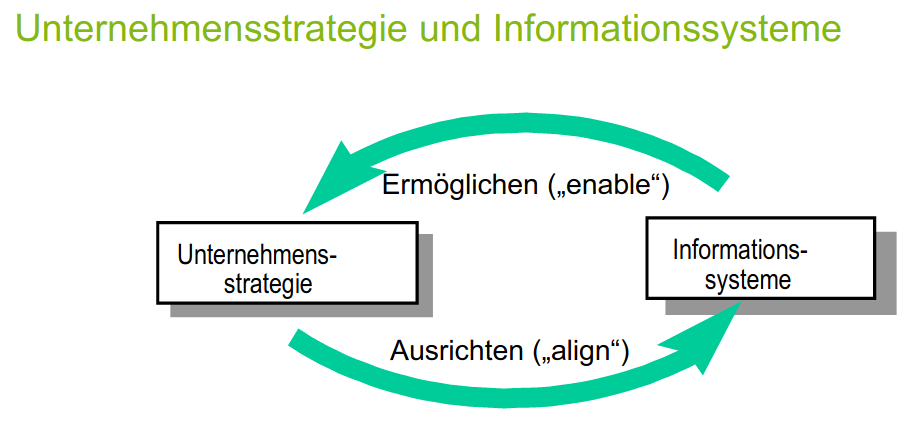
\includegraphics[scale=0.3]{UIS.png}
\\
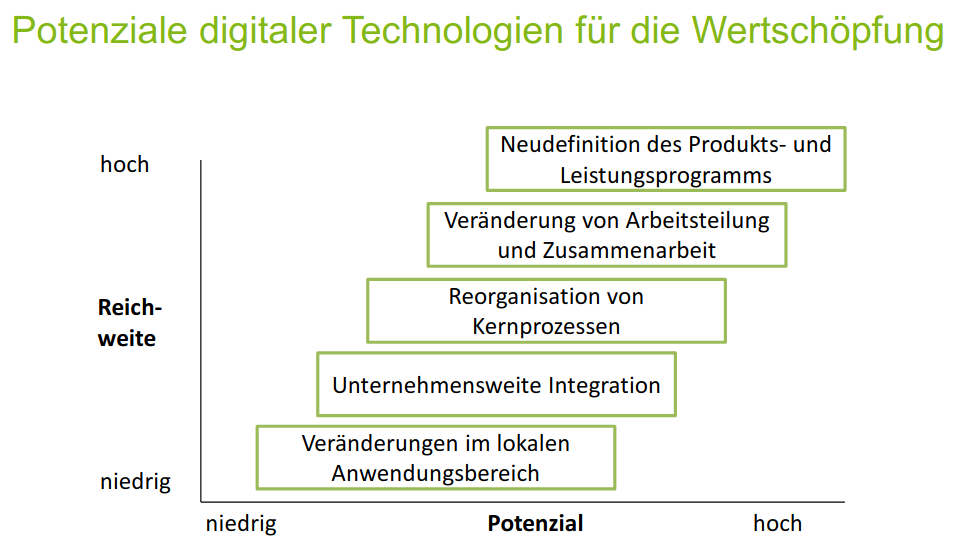
\includegraphics[scale=0.3]{Potenziale.png}



\end{document}